
In order to control ANSYS APDL in Python, an external library ansys-corba was used. During the analyses, ANSYS runs in a batch mode referred as "-aas" mode. Fig~\ref{fig:ansys_apdl_launching_scheme} describes how such a simulation should be launched in ANSYS APDL Product Launcher. Moreover, the Python script should run in the directory where the numerical simulation is conducted.

\begin{figure}[H]
    \centering
    \begin{tikzpicture}
    \node at (0,0) {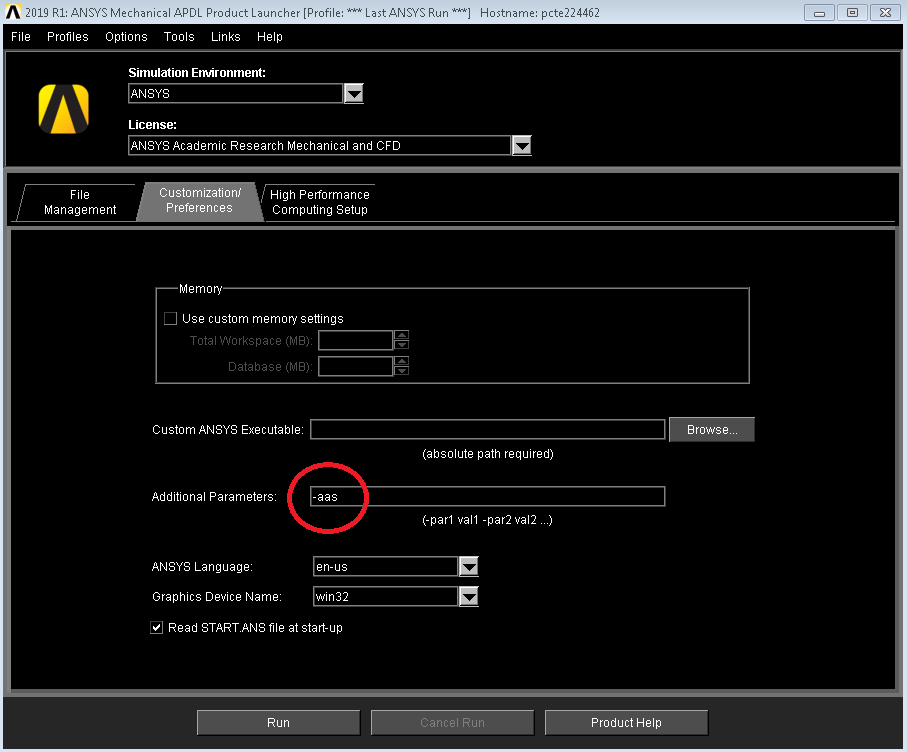
\includegraphics[width=.5\textwidth]{sections/appendices/analysis_in_python/ANSYS_APDL_launching_scheme.png}};
    \end{tikzpicture}
    \caption{ANSYS APDL launching scheme.}
    \label{fig:ansys_apdl_launching_scheme}
\end{figure}

The representative code for Python compilation with ANSYS environment is presented in Table~\ref{table:ansys_python_compilation}. By using the methods .executeCommandToString(), one can simply translate ANSYS APDL scripting commands into a Python language.

\begin{table}[H]
    \caption{Compilation of Python with ANSYS environment} 
    \vspace{-1em} 
    \fontsize{10}{10}
    \selectfont 
    \renewcommand{\arraystretch}{1}
    \begin{center}
    \begin{tabular}{ ll }  
    \hline  
        from ansys\_corba import CORBA & - imports ANSYS library \\
        os.chdir(directory) & - sets analysis directory\\
        with open('aaS\_MapdlID.txt', 'r') as f: \\ aasMapdlKey = f.read() & - opens APDL analysis \\
        mapdl = CORBA.ORB\_init().string\_to\_object(aasMapdlKey) & - creates mapdl object \\
    \hline
        mapdl.executeCommandToString("/prep7") & - exemplary command \\
     \end{tabular} 
    \end{center}  
     \label{table:ansys_python_compilation} 
 \end{table}
